\documentclass[journal]{IEEEtran}

\usepackage{amsmath,amssymb}
\usepackage{graphicx}
\usepackage{booktabs}
\usepackage{array}
\usepackage{multirow}
\usepackage{url}
\usepackage{cite}

\graphicspath{{raw_data/raw_data/}{figures/}}

\begin{document}

\title{A Residual Decomposition Framework with Attention-Based Sequence Modeling for Renewable Energy Forecasting and Blockchain-Anchored Scheduling}

\author{Ankit Subedi, Deepika J, Abhishek Kumar, and Liz Alex%
\thanks{Ankit Subedi is with the Department of Information Security, School of Computer Science and Engineering, VIT University, Vellore, Tamil Nadu, India.}%
\thanks{Deepika J is with the Department of Information Security, School of Computer Science and Engineering, VIT University, Vellore, Tamil Nadu, India. Corresponding author: Deepika J (e-mail: deepika.j@vit.ac.in).}%
\thanks{Abhishek Kumar is with the Department of Information Technology, School of Computer Science Engineering and Information Systems, VIT University, Vellore, Tamil Nadu, India.}%
\thanks{Liz Alex is with the Department of Computer Science Engineering, School of Computer Science and Engineering, VIT University, Vellore, Tamil Nadu, India.}}

\maketitle

\begin{abstract}
Accurate short-term renewable-energy forecasting is important for smart-grid operation because dispatch, storage, and renewable-aware scheduling decisions are sensitive to forecast error during high-variability periods. This paper presents a residual decomposition framework in which a multivariate Linear Regression (LR) model captures the dominant deterministic structure of hourly renewable generation, while a lightweight attention-based Bidirectional Long Short-Term Memory (BiLSTM) model is trained only on the residual error left by the linear component. The updated implementation uses 8760 hourly records derived from GridPath India renewable-resource data for Tamil Nadu, including fixed-tilt solar, single-axis solar, rooftop solar, adjusted onshore wind, engineered load, and storage-state features. A 48-hour lookback window with 10 input channels is used for sequence modeling. The revised evaluation shows that LR remains a very strong global baseline: on the current test split, LR obtains RMSE 0.006333, MAE 0.004678, and $R^2=0.988452$, while the hybrid residual model across five random seeds obtains RMSE $0.006918 \pm 0.001294$, MAE $0.005062 \pm 0.000847$, and $R^2=0.985837 \pm 0.005798$. A Diebold-Mariano test does not show statistically significant improvement of the hybrid model over LR on the full test set or on the peak subset where $y \ge 0.20$. The contribution of the residual architecture is therefore framed as interpretability, failure-mode analysis, and deployable decomposition rather than as a global accuracy win over LR. The blockchain component is presented as a proposed oracle architecture that serializes forecasts into canonical JSON, hashes payloads, and exposes deterministic scheduling gates; no gas-cost, consensus-latency, privacy, or production smart-contract benchmark is claimed. Under the same scheduling threshold of 0.15, LR and the hybrid model identify the same 280 eligible hours out of 1266 test hours and produce the same scheduled renewable share of 25.81 percent.
\end{abstract}

\begin{IEEEkeywords}
Attention mechanism, bidirectional LSTM, blockchain oracle, energy-aware scheduling, residual decomposition, renewable-energy forecasting, smart grid.
\end{IEEEkeywords}

\section{Introduction}
Renewable energy forecasting is now a core requirement for power-system operation because solar and wind output varies with weather, time of day, and season. As renewable penetration increases, grid operators must make dispatch, storage, and scheduling decisions under greater uncertainty. Forecast error during peak-generation or transition periods can lead to underutilized renewable energy, avoidable curtailment, larger reserve requirements, and inefficient downstream decisions.

This work studies short-term renewable forecasting for Tamil Nadu using a residual decomposition strategy. Instead of forcing a single nonlinear learner to model the entire target, the forecasting problem is split into two components. First, a Linear Regression model captures the dominant deterministic relationship between engineered renewable features and the target. Second, a compact attention-based BiLSTM is trained on the residual error:
\begin{equation}
e_t = y_t - \hat{y}^{LR}_t .
\end{equation}
The final prediction is
\begin{equation}
\hat{y}^{Hybrid}_t = \hat{y}^{LR}_t + \hat{e}^{BiLSTM}_t .
\end{equation}

The original manuscript emphasized improvement over Random Forest and standalone recurrent models. The updated notebook and priority review require a more precise claim. The revised evidence shows near-parity between LR and the residual hybrid on the main global metrics, with LR slightly stronger in the current repeated evaluation. The hybrid is therefore best interpreted as an architecture that makes the deterministic and stochastic portions of the problem explicit, provides a clear diagnostic route for nonlinear residuals, and offers a structured interface for forecast-gated scheduling.

The paper also includes a blockchain-facing design. In the revised manuscript, this component is explicitly treated as a proposed oracle architecture rather than a quantitatively benchmarked blockchain prototype. Forecast payloads can be serialized, hashed, and gated by smart contracts, but gas cost, consensus latency, privacy leakage, and adversarial robustness remain outside the empirical claims of this paper.

The main contributions are:
\begin{enumerate}
\item A residual decomposition framework that separates deterministic renewable-generation structure from localized residual deviations.
\item An attention-based BiLSTM residual learner that operates on 48-hour sequences after the linear component has already captured the dominant trend.
\item A statistical robustness update using peak-count reporting, Diebold-Mariano testing, and five random seeds.
\item A corrected scheduling interpretation that compares LR, hybrid residual forecasts, and perfect foresight under the same threshold rule.
\item A clarified blockchain-oracle formulation with an exact deterministic score definition and an explicit boundary between proposed architecture and evaluated system behavior.
\end{enumerate}

\section{Related Work}
Renewable-energy forecasting has been studied using statistical, physical, machine-learning, and deep-learning approaches. Classical time-series models such as ARIMA and SARIMA are interpretable when seasonal structure is stable, while machine-learning models can capture feature interactions without requiring a full physical model. Tree-based models such as Random Forest and gradient boosting are common nonlinear baselines but do not directly encode temporal order unless lagged windows are manually constructed.

Recurrent sequence models, including LSTM, GRU, and BiLSTM networks, are frequently used for energy forecasting because they can process historical sequences. However, when the target contains a large deterministic component, a standalone recurrent network may spend capacity relearning patterns that a simple linear model already captures. Residual learning addresses this problem by letting the nonlinear learner focus on the remaining error signal.

Attention mechanisms can assign different weights to time steps within a lookback window. Transformer-family models extend this idea with self-attention and have improved long-horizon forecasting in several domains. In this study, however, the available dataset is moderate in size and the linear baseline is already strong. The priority of the residual model is therefore compactness and interpretability, not transformer-scale capacity.

Blockchain-based energy systems have been explored for peer-to-peer energy markets, decentralized settlement, and smart contracts. Most such systems record meter reads, bids, or transactions after the fact. The present design instead describes how a forecast payload could become a verifiable control input. The revised paper does not claim a deployed blockchain benchmark; it specifies the oracle pathway needed for future implementation.

\section{Data and Feature Construction}
The dataset is derived from the GridPath India planning-data release. The notebook processes four capacity-factor sources:
\begin{itemize}
\item fixed-tilt solar PV,
\item single-axis tracking solar PV,
\item rooftop solar PV,
\item adjusted existing onshore wind.
\end{itemize}
Each source is filtered for Tamil Nadu and aggregated to hourly timestamps. The final master dataset contains 8760 hourly records from 2019 with no missing hourly intervals after validation. The current notebook adds rooftop solar consistently to the folder map and final schema.

Installed capacity and engineered operating variables are then used to construct generated power, load, storage state of charge, cyclical time features, and the forecasting target. The current target is log-transformed:
\begin{equation}
y_t = \log(1 + P^{gen}_t / P^{peak}),
\end{equation}
where $P^{gen}_t$ is modeled renewable generation and $P^{peak}$ is peak load. Hour-of-day and day-of-year are encoded as sine and cosine pairs to avoid artificial discontinuities at cyclic boundaries.

\begin{table}[!t]
\caption{Core Dataset and Modeling Configuration}
\label{tab:data_config}
\centering
\begin{tabular}{ll}
\toprule
Item & Value \\
\midrule
Hourly records & 8760 \\
Region & Tamil Nadu \\
Capacity-factor sources & 4 \\
Lookback window & 48 hours \\
Input channels & 10 \\
Test sequences & 1266 \\
Peak subset rule & $y \ge 0.20$ \\
Peak test points & 114 of 1266 (9.0 percent) \\
Scheduler threshold & 0.15 \\
\bottomrule
\end{tabular}
\end{table}

\section{Residual Decomposition Method}
\subsection{Linear Deterministic Component}
The LR baseline is trained on flattened 48-hour sequence windows. It acts as the deterministic anchor because the feature set contains strong diurnal, seasonal, and generation-load structure. In the current notebook, LR obtains the best deterministic global test metrics.

\subsection{Attention-Based BiLSTM Residual Learner}
The residual learner receives the same 48-hour feature window, but its target is the LR residual. The model uses a bidirectional LSTM layer with 16 hidden units per direction, an attention layer, dropout, a dense hidden layer, and a scalar residual output. This design keeps the nonlinear learner small and makes its role clear: it adjusts the linear forecast only where the residual signal provides useful information.

\subsection{Training Protocol}
The model is trained using Adam, mean-squared-error loss, validation MAE monitoring, early stopping with restored best weights, and reduce-on-plateau scheduling. The current notebook records the LR baseline as deterministic and repeats the hybrid training with five seeds: 42, 123, 456, 789, and 2024.

\begin{table}[!t]
\caption{Training Configuration}
\label{tab:training_config}
\centering
\begin{tabular}{ll}
\toprule
Parameter & Value \\
\midrule
Lookback & 48 hours \\
Residual learner & Attention-BiLSTM \\
BiLSTM units & 16 per direction \\
Dropout & 0.2 and 0.1 \\
Optimizer & Adam \\
Loss & MSE \\
Validation monitor & MAE / validation loss \\
Batch size & 64 \\
Maximum epochs & 200 in repeated evaluation \\
Seeds & 42, 123, 456, 789, 2024 \\
\bottomrule
\end{tabular}
\end{table}

\section{Forecasting Results}
\subsection{Global Baseline Comparison}
Table~\ref{tab:global_baselines} reports the updated baseline metrics from the notebook's log-scale evaluation. LR is the strongest global baseline, Random Forest is weaker, and the hybrid residual model is statistically close but not better than LR in the current repeated evidence.

\begin{table}[!t]
\caption{Updated Global Test Metrics}
\label{tab:global_baselines}
\centering
\begin{tabular}{lccc}
\toprule
Model & RMSE & MAE & $R^2$ \\
\midrule
Linear Regression & 0.006333 & 0.004678 & 0.988452 \\
Random Forest & 0.008497 & 0.006007 & 0.979212 \\
Hybrid, five-seed mean & 0.006918 & 0.005062 & 0.985837 \\
Hybrid, five-seed std. & 0.001294 & 0.000847 & 0.005798 \\
\bottomrule
\end{tabular}
\end{table}

These results revise the original interpretation. The residual model should not be described as outperforming LR on global metrics. It remains competitive with LR and better motivated as a decomposed, auditable model that separates deterministic structure from residual deviations.

\subsection{Single-Run Metrics Matching the Earlier Manuscript}
The earlier manuscript reported a single-run comparison in which LR and the hybrid model were nearly identical, while Random Forest was weaker. That result is retained only as a historical single-run output, not as the final robustness claim.

\begin{table}[!t]
\caption{Historical Single-Run Metrics from Earlier Notebook Cells}
\label{tab:single_run}
\centering
\begin{tabular}{lccc}
\toprule
Model & Test RMSE & Test MAE & Test $R^2$ \\
\midrule
Linear Regression & 0.007334 & 0.005305 & 0.988058 \\
Hybrid error correction & 0.007337 & 0.005312 & 0.988051 \\
Random Forest & 0.009822 & 0.006824 & 0.978584 \\
\bottomrule
\end{tabular}
\end{table}

\subsection{Peak-Generation Subset}
The priority review requested explicit sample-count support for peak claims. Using $y \ge 0.20$, the peak subset contains 114 test points out of 1266, or 9.0 percent. On this subset, LR and the hybrid model are again near-tied, with LR slightly lower in RMSE and MAE.

\begin{table}[!t]
\caption{Peak-Subset Comparison, $y \ge 0.20$}
\label{tab:peak_subset}
\centering
\begin{tabular}{lcc}
\toprule
Metric & Linear Regression & Hybrid \\
\midrule
Peak points & \multicolumn{2}{c}{114 of 1266} \\
Peak RMSE & 0.009724 & 0.009738 \\
Peak MAE & 0.007502 & 0.007508 \\
RMSE improvement & \multicolumn{2}{c}{-0.14 percent} \\
MAE improvement & \multicolumn{2}{c}{-0.08 percent} \\
\bottomrule
\end{tabular}
\end{table}

\subsection{Diebold-Mariano Significance Test}
The Diebold-Mariano (DM) test compares the predictive accuracy of LR and the hybrid model using loss differentials. Positive loss differential means the hybrid model is better. The current test does not show significant improvement for the hybrid model on either full-test or peak-test evaluation.

\begin{table}[!t]
\caption{Diebold-Mariano Test: LR vs. Hybrid}
\label{tab:dm_test}
\centering
\begin{tabular}{llccc}
\toprule
Subset & Loss & $n$ & DM stat. & $p$-value \\
\midrule
Full test & Squared & 1266 & -0.2139 & 0.8307 \\
Full test & Absolute & 1266 & -0.3199 & 0.7491 \\
Peak $y \ge 0.20$ & Squared & 114 & -0.5246 & 0.6009 \\
\bottomrule
\end{tabular}
\end{table}

The negative DM statistics indicate that LR has slightly lower average loss in these comparisons, although the differences are not statistically significant at $\alpha=0.05$.

\subsection{Repeated-Seed Robustness}
Table~\ref{tab:seed_results} summarizes five hybrid training runs. Only one seed produces a significant DM result at $p<0.05$, and the average DM statistic remains negative. Therefore, the revised conclusion is that the hybrid model achieves near-parity but does not consistently outperform LR.

\begin{table}[!t]
\caption{Hybrid Residual Model Across Five Seeds}
\label{tab:seed_results}
\centering
\begin{tabular}{rccccc}
\toprule
Seed & RMSE & MAE & $R^2$ & Peak RMSE & DM $p$ \\
\midrule
42 & 0.006376 & 0.004715 & 0.988296 & 0.009734 & 0.4360 \\
123 & 0.006335 & 0.004683 & 0.988444 & 0.009728 & 0.8879 \\
456 & 0.009231 & 0.006577 & 0.975467 & 0.011001 & 0.0627 \\
789 & 0.006347 & 0.004690 & 0.988403 & 0.009721 & 0.0136 \\
2024 & 0.006299 & 0.004647 & 0.988576 & 0.009749 & 0.0960 \\
\bottomrule
\end{tabular}
\end{table}

\begin{figure}[!t]
\centering
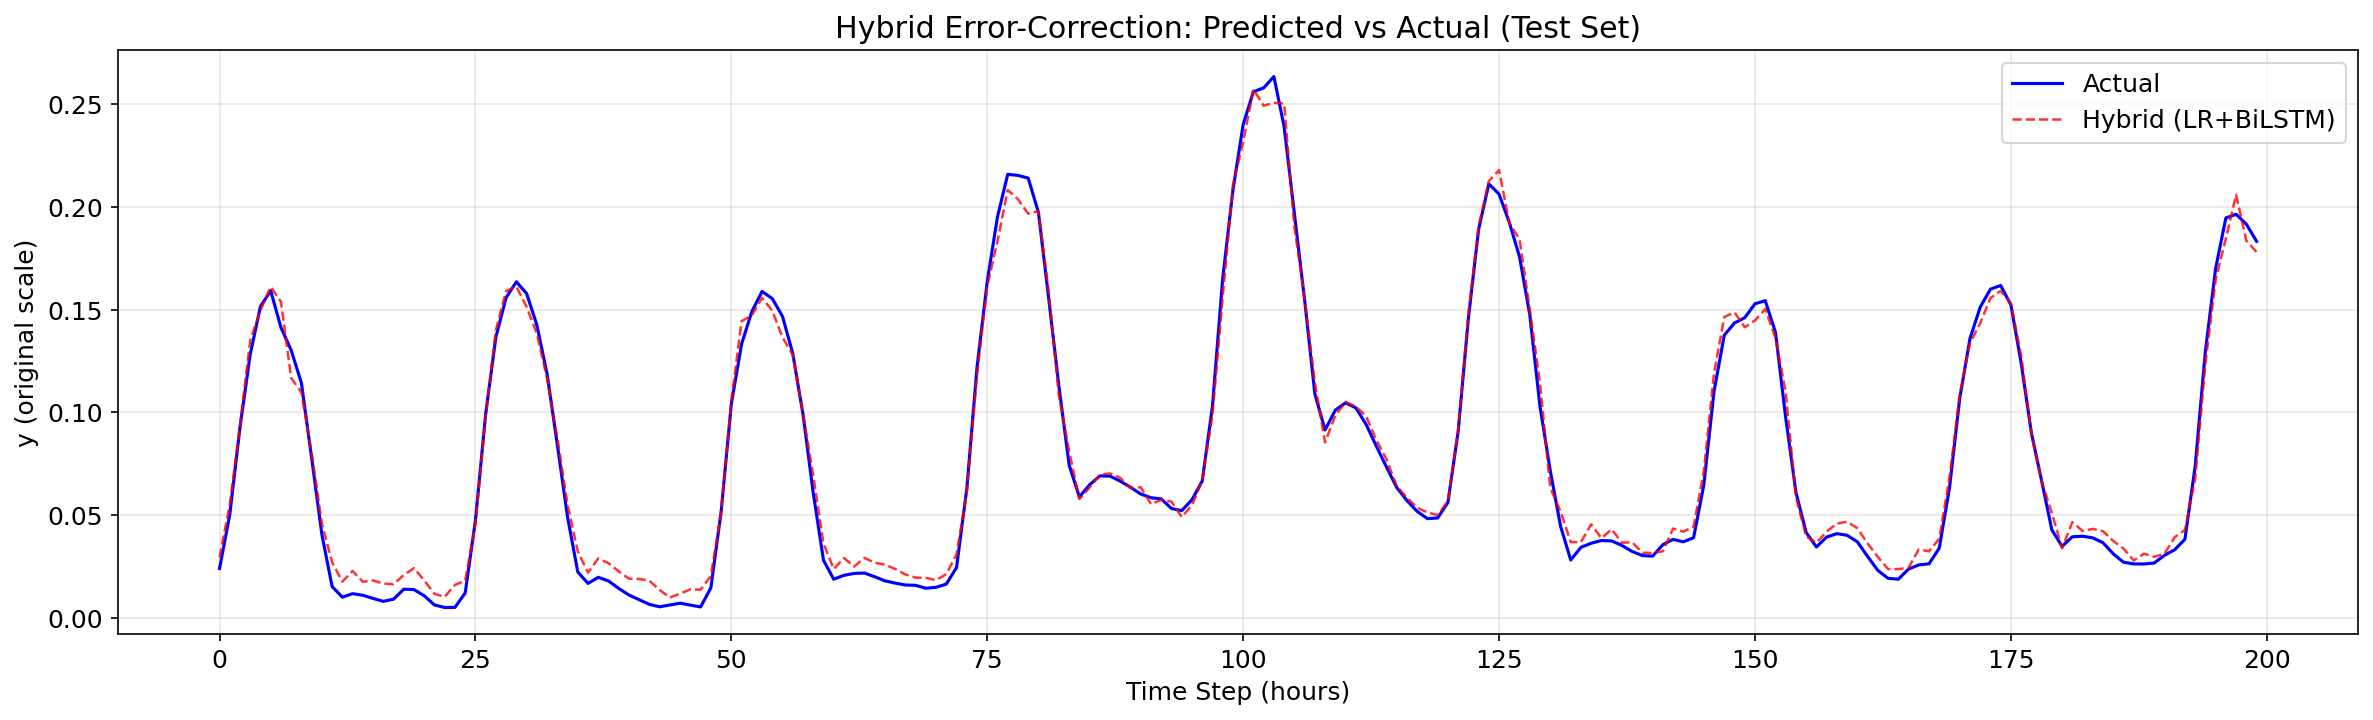
\includegraphics[width=\linewidth]{prediction_vs_actual.png}
\caption{Prediction versus actual renewable target from the model-comparison output. The revised interpretation is near-parity between LR and the hybrid model, not a consistent hybrid win over LR.}
\label{fig:prediction_actual}
\end{figure}

\begin{figure}[!t]
\centering
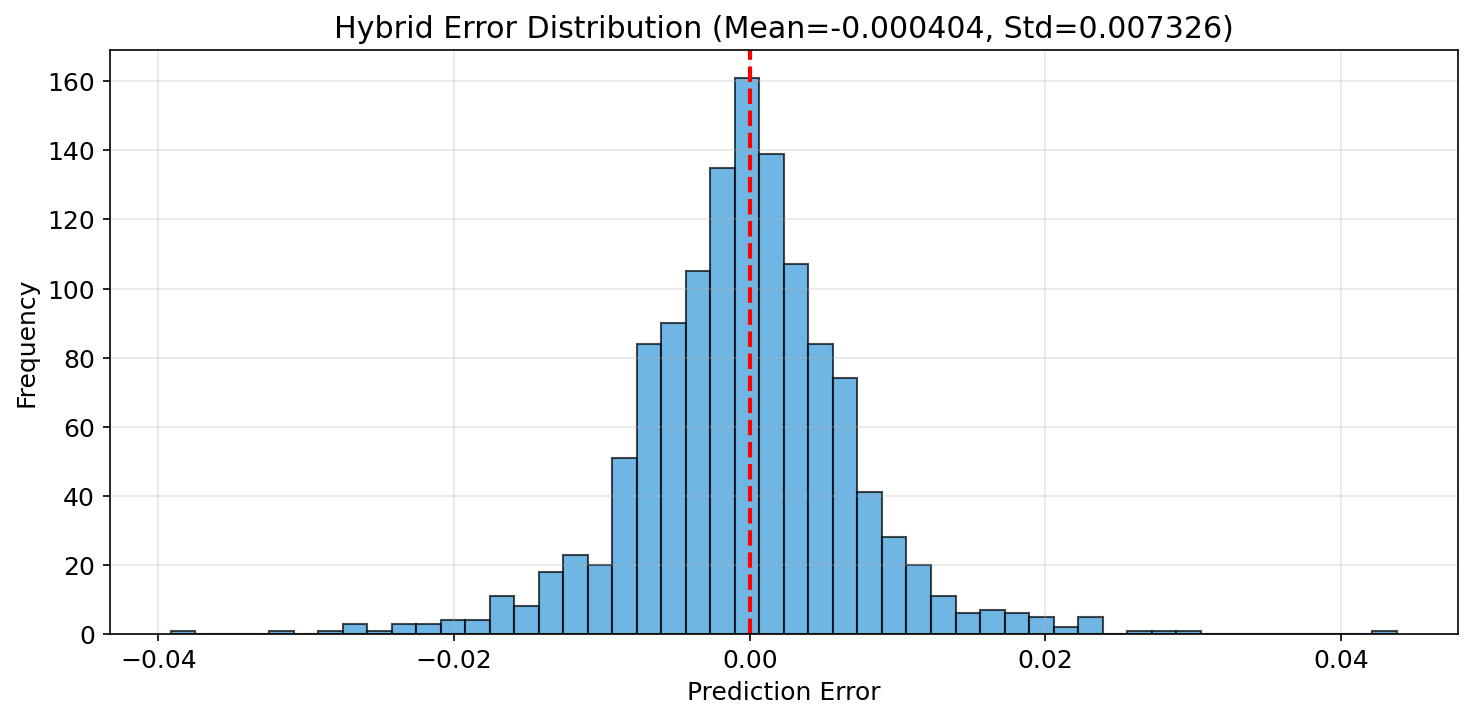
\includegraphics[width=\linewidth]{error_distribution.png}
\caption{Error distribution from the notebook output. Residual tails motivate residual diagnostics, but the statistical tests do not establish a significant hybrid improvement over LR.}
\label{fig:error_distribution}
\end{figure}

\section{Residual Diagnostics}
The residual analysis shows why the decomposition is still useful even when LR is globally strong. LR tracks the main trajectory closely, but localized residual spikes occur around transition and high-generation periods. The top 5 percent absolute LR residuals contain 64 of 1266 test points. These points motivate residual monitoring and targeted model refinement, but the revised paper avoids claiming that the current hybrid model has already solved these cases better than LR.

\begin{figure}[!t]
\centering
\includegraphics[width=\linewidth]{stage4_test_predictions_first168h.png}
\caption{First 168 hours of test predictions. The figure is retained as a visual diagnostic for localized error behavior.}
\label{fig:first168}
\end{figure}

\section{Blockchain Oracle and Scheduling Architecture}
\subsection{Revised Scope of the Blockchain Component}
The blockchain component is now explicitly scoped as a proposed oracle architecture. The revised manuscript does not claim a production smart-contract deployment, gas-cost benchmark, consensus-latency benchmark, privacy analysis, or adversarial security evaluation. Instead, it defines the data path by which forecasts can be made auditable:
\begin{equation}
\text{forecast} \rightarrow \text{canonical JSON} \rightarrow \text{hash/CID} \rightarrow \text{ledger anchor} \rightarrow \text{scheduling gate}.
\end{equation}

This framing resolves the inconsistency between describing IPFS/CID anchoring and simultaneously listing gas cost, latency, privacy, and consensus evaluation as future work.

\subsection{Forecast Payload}
Each payload contains a timestamp, model identifier, predicted renewable target, scheduling threshold, feature-window metadata, and a deterministic hash of the canonical JSON serialization. The ledger stores only the digest and minimal metadata, while the full payload can be stored off-chain.

\subsection{Predictive Green Score}
The original manuscript used both a 0--100 confidence score and a 7000/10000 on-chain threshold. The revised definition removes that inconsistency. The empirical scheduler uses a normalized forecast threshold $\tau_s=0.15$. For on-chain integer representation, the Predictive Green Score (PGS) is defined as
\begin{equation}
PGS_t = \operatorname{round}\left(10000 \cdot \operatorname{clip}(\hat{y}_t,0,1)\right),
\end{equation}
where $\hat{y}_t$ is the normalized forecast used by the scheduler. The empirical scheduling gate is therefore
\begin{equation}
E_t = \mathbb{1}[\hat{y}_t \ge 0.15] = \mathbb{1}[PGS_t \ge 1500].
\end{equation}
This is a deterministic forecast-strength score, not a calibrated probabilistic confidence score. Calibrated uncertainty-aware PGS design remains future work.

\subsection{Scheduling Evaluation}
The previous scheduling section attributed renewable-share improvement to the proposed model. The revised notebook applies the same 0.15 threshold to LR, the hybrid model, and perfect foresight. LR and the hybrid select the same 280 eligible hours and obtain the same scheduled renewable share. Perfect foresight selects 290 hours and obtains a similar renewable share. Therefore, the scheduling gain is attributed primarily to the thresholded selection rule under this dataset, not to a demonstrated forecast-quality advantage of the hybrid over LR.

\begin{table}[!t]
\caption{Scheduling Metrics for the Original Thresholded Run}
\label{tab:scheduling_metrics}
\centering
\begin{tabular}{lc}
\toprule
Metric & Value \\
\midrule
Total test hours & 1266 \\
Eligible hours & 280 \\
Blocked hours & 986 \\
Allowed hours & 22.12 percent \\
Always-on renewable share & 15.34 percent \\
Scheduled renewable share & 25.81 percent \\
Improvement & 10.47 percentage points \\
Relative improvement & 68.26 percent \\
\bottomrule
\end{tabular}
\end{table}

\begin{table}[!t]
\caption{Same 0.15 Scheduling Rule Across Forecast Sources}
\label{tab:scheduling_comparison}
\centering
\begin{tabular}{lccc}
\toprule
Forecast source & Eligible hours & Eligible pct. & Renewable share \\
\midrule
Linear Regression & 280 & 22.12 & 25.81 percent \\
Hybrid LR+BiLSTM & 280 & 22.12 & 25.81 percent \\
Perfect foresight & 290 & 22.91 & 25.74 percent \\
\bottomrule
\end{tabular}
\end{table}

\section{Discussion}
\subsection{What the Revised Evidence Supports}
The evidence supports three main conclusions. First, LR is an unusually strong baseline for this feature construction because the target is closely related to generated power and cyclical structure. Second, residual decomposition remains valuable as an interpretable modeling design because it makes clear which part of the forecast is deterministic and which part is a learned correction. Third, the scheduling layer is useful as a renewable-aware decision rule, but current results do not prove that the hybrid model improves scheduling outcomes over LR.

\subsection{What the Revised Evidence Does Not Support}
The revised evidence does not support claiming that the hybrid model significantly outperforms LR on global RMSE, MAE, $R^2$, or peak-subset RMSE. It also does not support claiming that blockchain deployment has been quantitatively evaluated. Finally, the old ``optimized oracle export'' result is removed from the central claims because the mechanism and metric scale are not sufficiently defined in the current manuscript assets.

\subsection{Naming Consistency}
The model is referred to consistently as the \emph{hybrid residual model} or \emph{LR+attention-BiLSTM residual model}. Historical labels such as EA-BiLSTM are restricted to historical standalone variants and are not used as names for the final model.

\section{Conclusion}
This paper revises a residual decomposition approach for renewable-energy forecasting and forecast-gated scheduling. The updated notebook shows that Linear Regression is the strongest global baseline in the current evaluation, while the LR+attention-BiLSTM residual model achieves near-parity but does not consistently or significantly outperform LR. The revised contribution is therefore not a claim of global metric superiority; it is a clearer decomposition framework that separates deterministic structure from residual deviations, supports failure-mode analysis, and exposes a structured interface for scheduling decisions.

The scheduling results show that a 0.15 threshold selects 280 of 1266 hours and increases renewable share from 15.34 percent in the always-on baseline to 25.81 percent during scheduled windows. However, because LR and the hybrid model produce the same scheduling outcome under this rule, the operational gain is attributed to thresholded selection rather than to a demonstrated hybrid forecast advantage. The blockchain component is retained as a proposed oracle architecture with deterministic payload hashing and integer score representation, while production blockchain evaluation remains future work.

\section*{Declarations}
\textbf{Funding:} The authors declare that no external funding was received for this work.

\textbf{Conflicts of Interest:} The authors declare no conflicts of interest.

\textbf{Data Availability:} The raw renewable resource data are available from the GridPath India dataset on Dryad. Processed project artifacts used for this manuscript are maintained in the project workspace under \texttt{raw\_data/raw\_data}.

\textbf{Ethical Approval:} This study uses publicly available energy-system data and does not involve human participants or animal subjects.

\textbf{Author Contributions:} Abhishek Kumar, Ankit Subedi, and Liz Alex contributed to data preprocessing, model experimentation, system evaluation, and manuscript preparation. Deepika J supervised the work, reviewed the methodology, and served as corresponding author.

\section*{Acknowledgment}
The authors thank the School of Computer Science and Engineering, VIT University, Vellore, for providing the academic infrastructure and research environment that supported this work.

\begin{thebibliography}{99}

\bibitem{gridpath}
GridPath India long-term (2020--2050) power system planning model data, Dryad, doi: 10.5061/dryad.dz08kpsbm.

\bibitem{breiman}
L. Breiman, ``Random forests,'' \emph{Machine Learning}, vol. 45, no. 1, pp. 5--32, 2001.

\bibitem{hochreiter}
S. Hochreiter and J. Schmidhuber, ``Long short-term memory,'' \emph{Neural Computation}, vol. 9, no. 8, pp. 1735--1780, 1997.

\bibitem{schuster}
M. Schuster and K. K. Paliwal, ``Bidirectional recurrent neural networks,'' \emph{IEEE Transactions on Signal Processing}, vol. 45, no. 11, pp. 2673--2681, 1997.

\bibitem{bahdanau}
D. Bahdanau, K. Cho, and Y. Bengio, ``Neural machine translation by jointly learning to align and translate,'' in \emph{Proc. ICLR}, 2015.

\bibitem{vaswani}
A. Vaswani et al., ``Attention is all you need,'' in \emph{Proc. NeurIPS}, 2017, pp. 5998--6008.

\bibitem{he}
K. He, X. Zhang, S. Ren, and J. Sun, ``Deep residual learning for image recognition,'' in \emph{Proc. CVPR}, 2016, pp. 770--778.

\bibitem{pedregosa}
F. Pedregosa et al., ``Scikit-learn: Machine learning in Python,'' \emph{Journal of Machine Learning Research}, vol. 12, pp. 2825--2830, 2011.

\bibitem{kingma}
D. P. Kingma and J. Ba, ``Adam: A method for stochastic optimization,'' in \emph{Proc. ICLR}, 2015.

\bibitem{prechelt}
L. Prechelt, ``Early stopping: But when?'' in \emph{Neural Networks: Tricks of the Trade}. Berlin, Germany: Springer, 1998, pp. 55--69.

\bibitem{srivastava}
N. Srivastava, G. Hinton, A. Krizhevsky, I. Sutskever, and R. Salakhutdinov, ``Dropout: A simple way to prevent neural networks from overfitting,'' \emph{Journal of Machine Learning Research}, vol. 15, pp. 1929--1958, 2014.

\bibitem{tensorflow}
M. Abadi et al., ``TensorFlow: Large-scale machine learning on heterogeneous systems,'' 2015. [Online]. Available: \url{https://www.tensorflow.org/}

\bibitem{keras}
F. Chollet et al., ``Keras,'' 2015. [Online]. Available: \url{https://keras.io/}

\bibitem{andoni}
M. Andoni et al., ``Blockchain technology in the energy sector: A systematic review of challenges and opportunities,'' \emph{Renewable and Sustainable Energy Reviews}, vol. 100, pp. 143--174, 2019.

\bibitem{albreiki}
H. Al-Breiki, M. H. U. Rehman, K. Salah, and D. Svetinovic, ``Trustworthy blockchain oracles: Review, comparison, and open research challenges,'' \emph{IEEE Access}, vol. 8, pp. 85675--85685, 2020.

\bibitem{chainlink}
S. Ellis, A. Juels, and S. Nazarov, ``ChainLink: A decentralized oracle network,'' white paper, 2017.

\end{thebibliography}

\end{document}
